\section{Gestión de Unidades de Aprendizaje}
    \subsection{Consulta de Unidades de Aprendizaje}
Para consultar Unidades de Aprendizaje el Jefe de Departamento de Desarrollo e Innovación Curricular selecciona un Plan de Estudios en la pantalla \hyperlink{consultarS}{\textit{Consultar Planes de Estudios}}:\\
\begin{figure}[H]
    \centering
    \hypertarget{consultarS}{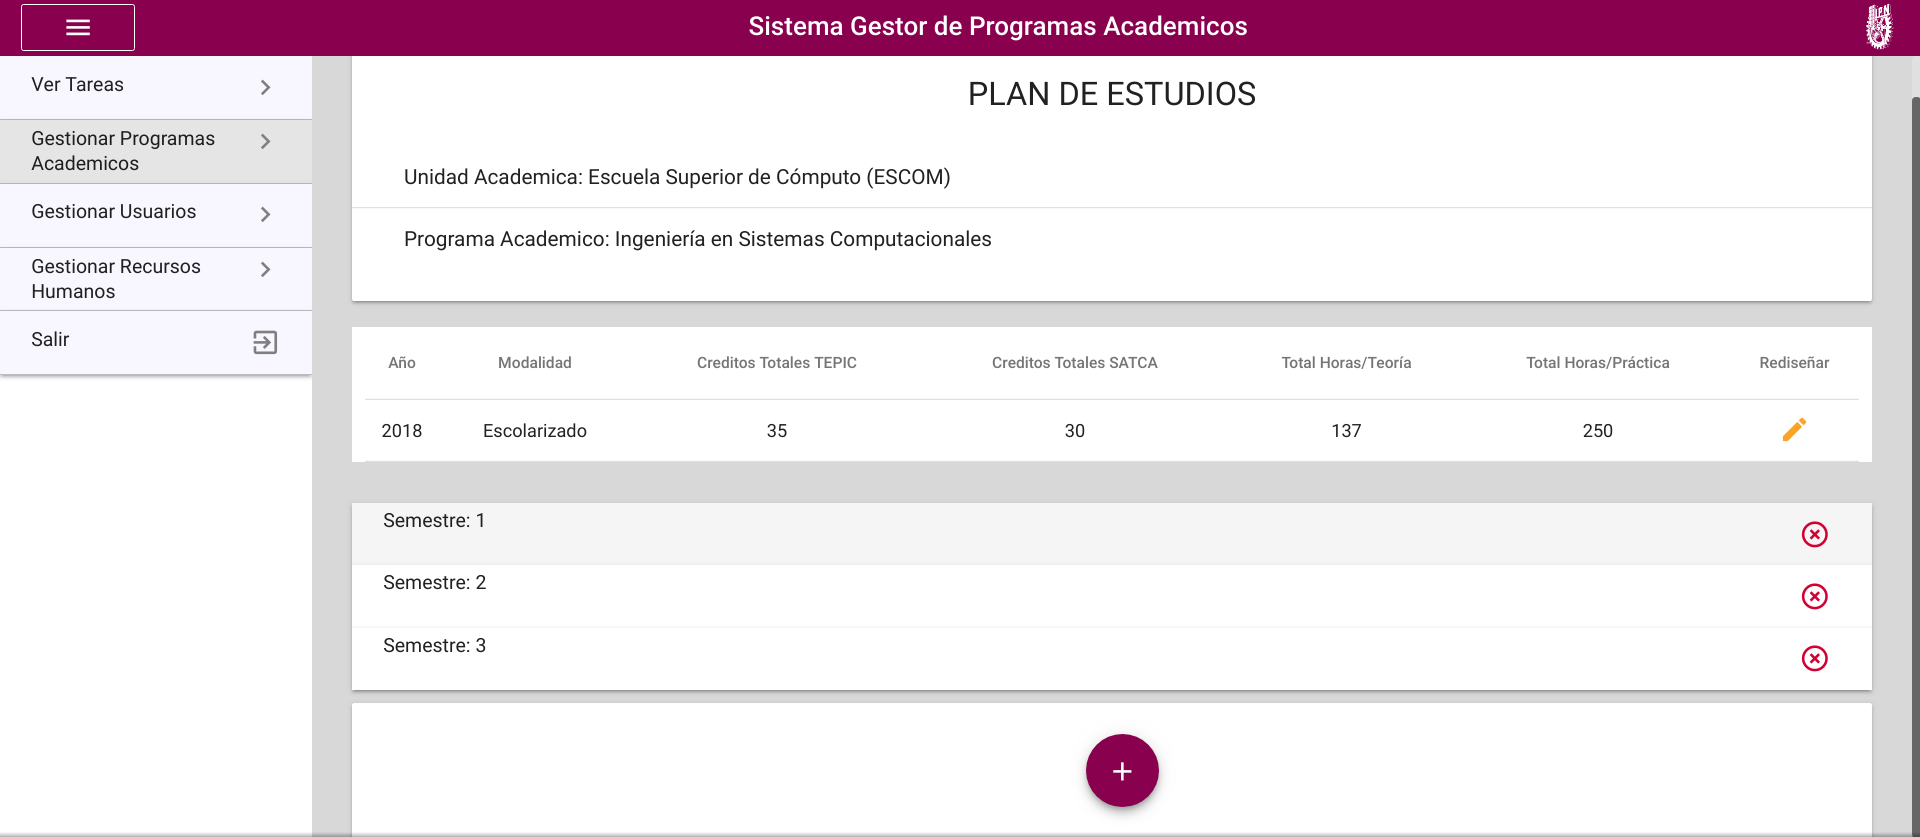
\includegraphics[width=0.7\linewidth]{images/GUA/consultarS}}
    \caption{Pantalla Consultar Plan de Estudios}
    \label{consultarS}
\end{figure}
\newpage
Una vez en esa pantalla presiona un semestre desplegando las Unidades de Aprendizaje que tiene asociadas, como se muestra en la pantalla \hyperlink{consultarUA}{\textit{Consultar Planes de Estudios}}:\\
\begin{figure}[H]
    \centering
    \hypertarget{consultarUA}{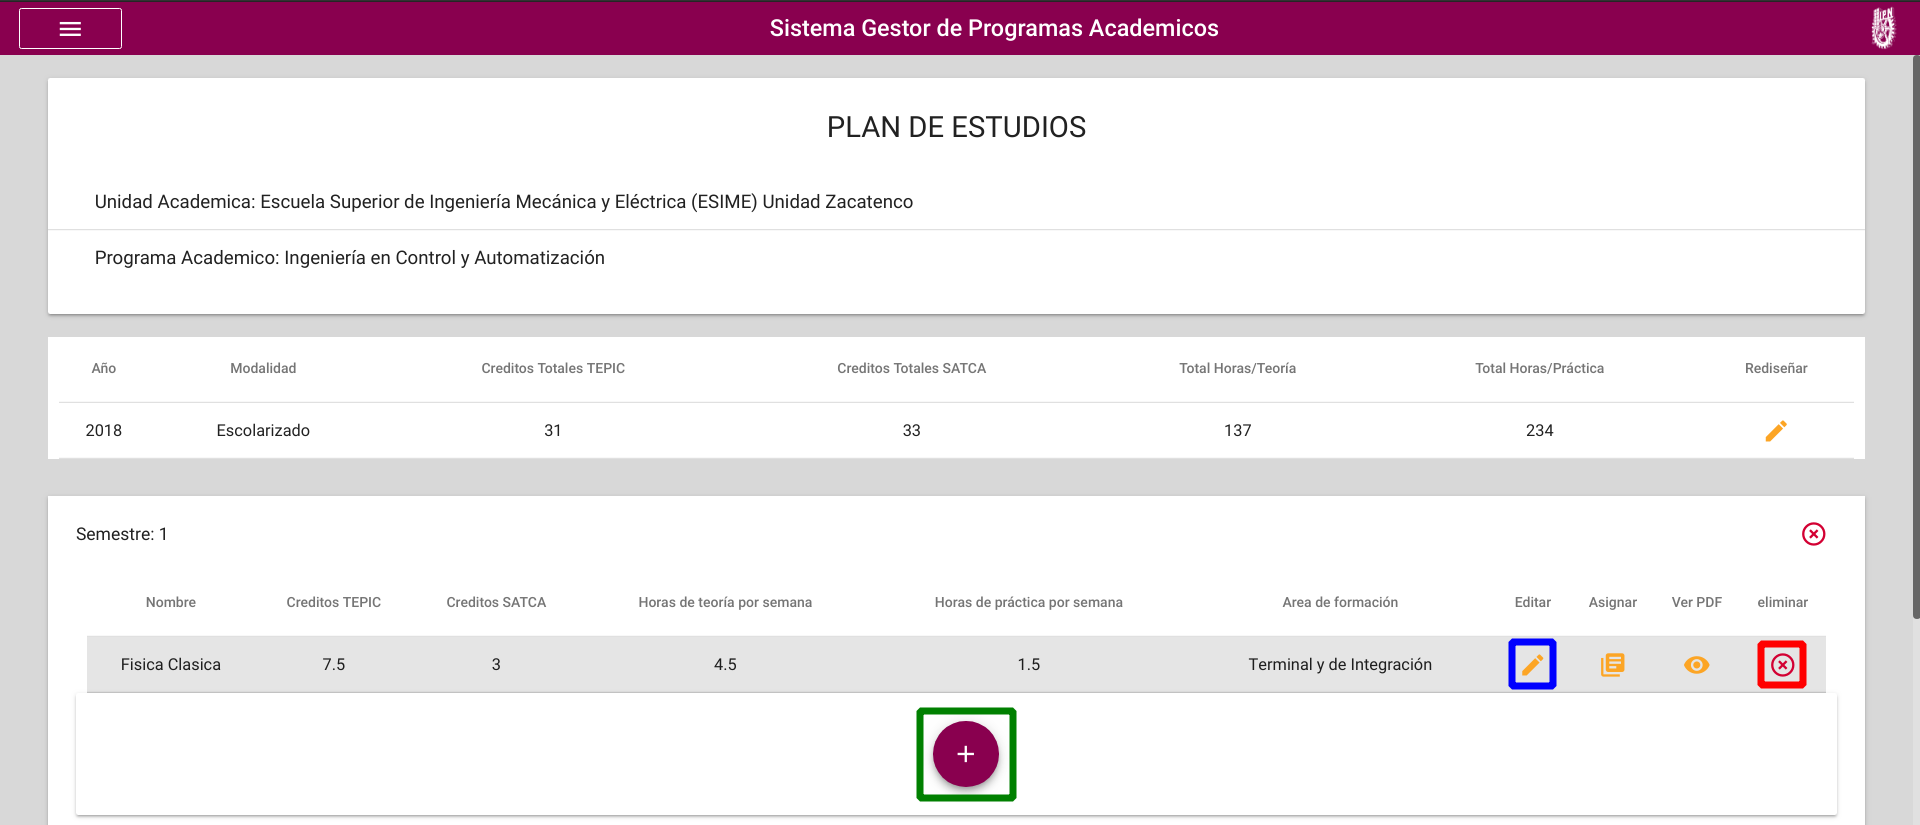
\includegraphics[width=0.7\linewidth]{images/GUA/consultarUA}}
    \caption{Pantalla Consultar Plan de Estudios Semestre expandido}
    \label{consultarUA}
\end{figure}
En esta ultima pantalla el usuario puede realizar las tareas relacionadas a la gestión de Unidades de Aprendizaje, Registrar Unidad de Aprendizaje (verde), Editar Unidad de Aprendizaje (azul) y Eliminar Unidad de Aprendizaje (rojo).
\newpage
\subsection{Agregar Semestres}
Cuando el usuario presiona el botón \IUbutton{+} de la pantalla \hyperlink{consultarS}{\textit{Consultar Planes de Estudios}} se agrega un nuevo Semestre, a menos que ya existan 8 semestres en ese caso se muestra el siguiente mensaje:
\begin{figure}[H]
    \centering
    \hypertarget{maxSemestres}{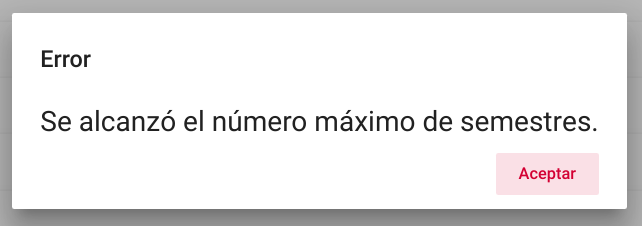
\includegraphics[width=0.7\linewidth]{images/GUA/maxSemestres}}
    \caption{Maximo de Semestres: aparece cuando se intenta agregar un noveno semestre.}
    \label{maxSemestres}
\end{figure}
\newpage
\subsection{Eliminar Semestres}
Cuando el usuario presiona el botón \IUbutton{X} de la pantalla \hyperlink{consultarS}{\textit{Consultar Planes de Estudios}} y el semestre seleccionado no cuenta con ninguna Unidad de Aprendizaje asociada se muestra el siguiente mensaje:
\begin{figure}[H]
    \centering
    \hypertarget{eliminarS}{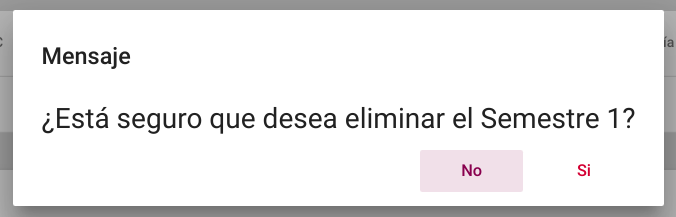
\includegraphics[width=0.7\linewidth]{images/GUA/eliminarS}}
    \caption{Eliminar Semestre: solicita confirmación para eliminar permanentemente un Semestre}
    \label{eliminarS}
\end{figure}
En caso que el semestre si este asociado a alguna Unidad de Aprendizaje se muestra este otro:
\begin{figure}[H]
    \centering
    \hypertarget{errorEliminarS}{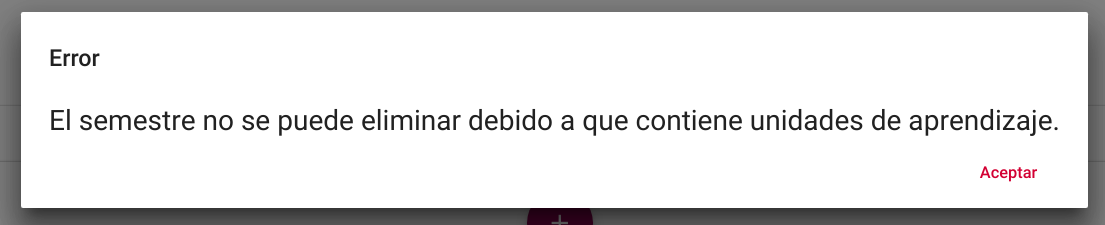
\includegraphics[width=0.7\linewidth]{images/GUA/errorEliminarS}}
    \caption{Imposibilidad de Eliminar: este mensaje aparece cuando se intenta eliminar a un Semestre con Unidades de Aprendizaje asociadas.}
    \label{errorEliminarS}
\end{figure}
\newpage
\subsection{Registrar Unidades de Aprendizaje}
Cuando el usuario presiona el botón \IUbutton{+}, el recuadro verde, en la pantalla \hyperlink{consultarUA}{\textit{Consultar Planes de Estudios}} se le redirecciona a la pantalla \hyperlink{registrarUA}{\textit{Registrar Unidad de Aprendizaje}}:\\
\begin{figure}[H]
    \centering
    \hypertarget{registrarUA}{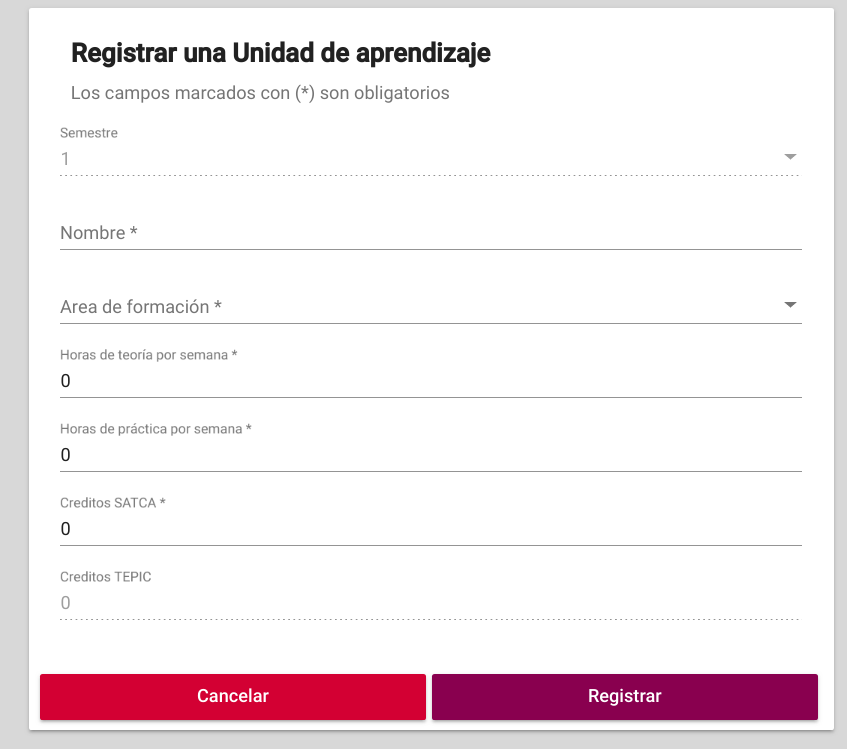
\includegraphics[width=0.7\linewidth]{images/GUA/registrarUA}}
    \caption{Pantalla Registrar Unidad de Aprendizaje}
    \label{registrarUA}
\end{figure}
\newpage
En donde ingresa los datos solicitados para registrar una nueva Unidad de Aprendizaje.\\
Cuando ingresa un dato que no cumple con el formato establecido el sistema se lo indica con el siguiente mensaje:\\
\begin{figure}[H]
    \centering
    \hypertarget{invalidoR}{
\includegraphics[width=0.7\linewidth]{images/GUA/invalido}}
    \caption{Campo inválido: aparece cuando el formato o el tipo de dato es incorrecto}
    \label{invalidoR}
\end{figure}
Si intenta finalizar o saltar sin haber llenado alguno de los campos  obligatorios, es decir marcados con (*), el sistema le muestra el siguiente mensaje:\\
\begin{figure}[H]
    \centering
    \hypertarget{requeridoR}{
\includegraphics[width=0.7\linewidth]{images/GUA/requerido}}
    \caption{Campo requerido: aparece cuando un campo obligatorio se dejo vacío}
    \label{requeridoR}
\end{figure}
Cuando desea finalizar el registro debe presionar el botón \IUbutton{Registrar}, que se encuentra en la parte inferior de la pantalla.\\
\begin{figure}[H]
    \centering
    \hypertarget{registrarBtnR}{
\includegraphics[width=0.7\linewidth]{images/GUA/registrarBtn}}
    \caption{Botones para finalizar o cancelar el registro}
    \label{registrarBtnR}
\end{figure}
Si la operación se pudo realizar aparece el siguiente mensaje:\\
\begin{figure}[H]
    \centering
    \hypertarget{exito}{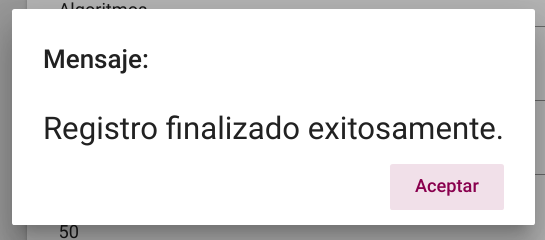
\includegraphics[width=0.7\linewidth]{images/GUA/exito}}
    \caption{Regisro Exitoso: aparece cuando su registro finaliza sin errores}
    \label{exito}
\end{figure}
En el caso de que haya ocurrido un error aparece este otro:\\
\begin{figure}[H]
    \centering
    \hypertarget{errorR}{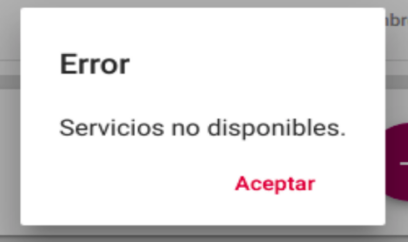
\includegraphics[width=0.7\linewidth]{images/GUA/error}}
    \caption{Error: Servicios no disponibles, aparece cuando ocurre un error en la conexión}
    \label{errorR}
\end{figure}
Si el usuario desea cancelar la operación debe presionar el botón \IUbutton{Cancelar} y se muestra el siguiente mensaje solicitando confirmación:\\
\begin{figure}[H]
    \centering
    \hypertarget{cancelarR}{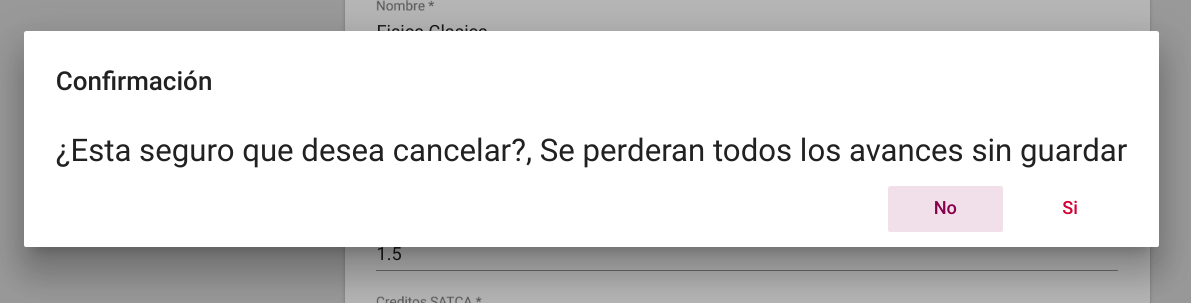
\includegraphics[width=0.7\linewidth]{images/GUA/cancelar}}
    \caption{Cancelación: permite finalizar la operacion sin guardar}
    \label{cancelarR}
\end{figure}
\newpage
\subsection{Editar Unidades de Aprendizaje}
Cuando el usuario presiona el botón \BtnLapiz, el recuadro azul, en la pantalla \hyperlink{consultarUA}{\textit{Consultar Planes de Estudios}} se le redicciona a la pantalla \hyperlink{editarUA}{\textit{Editar Unidad de Aprendizaje}}:\\
\begin{figure}[H]
    \centering
    \hypertarget{editarUA}{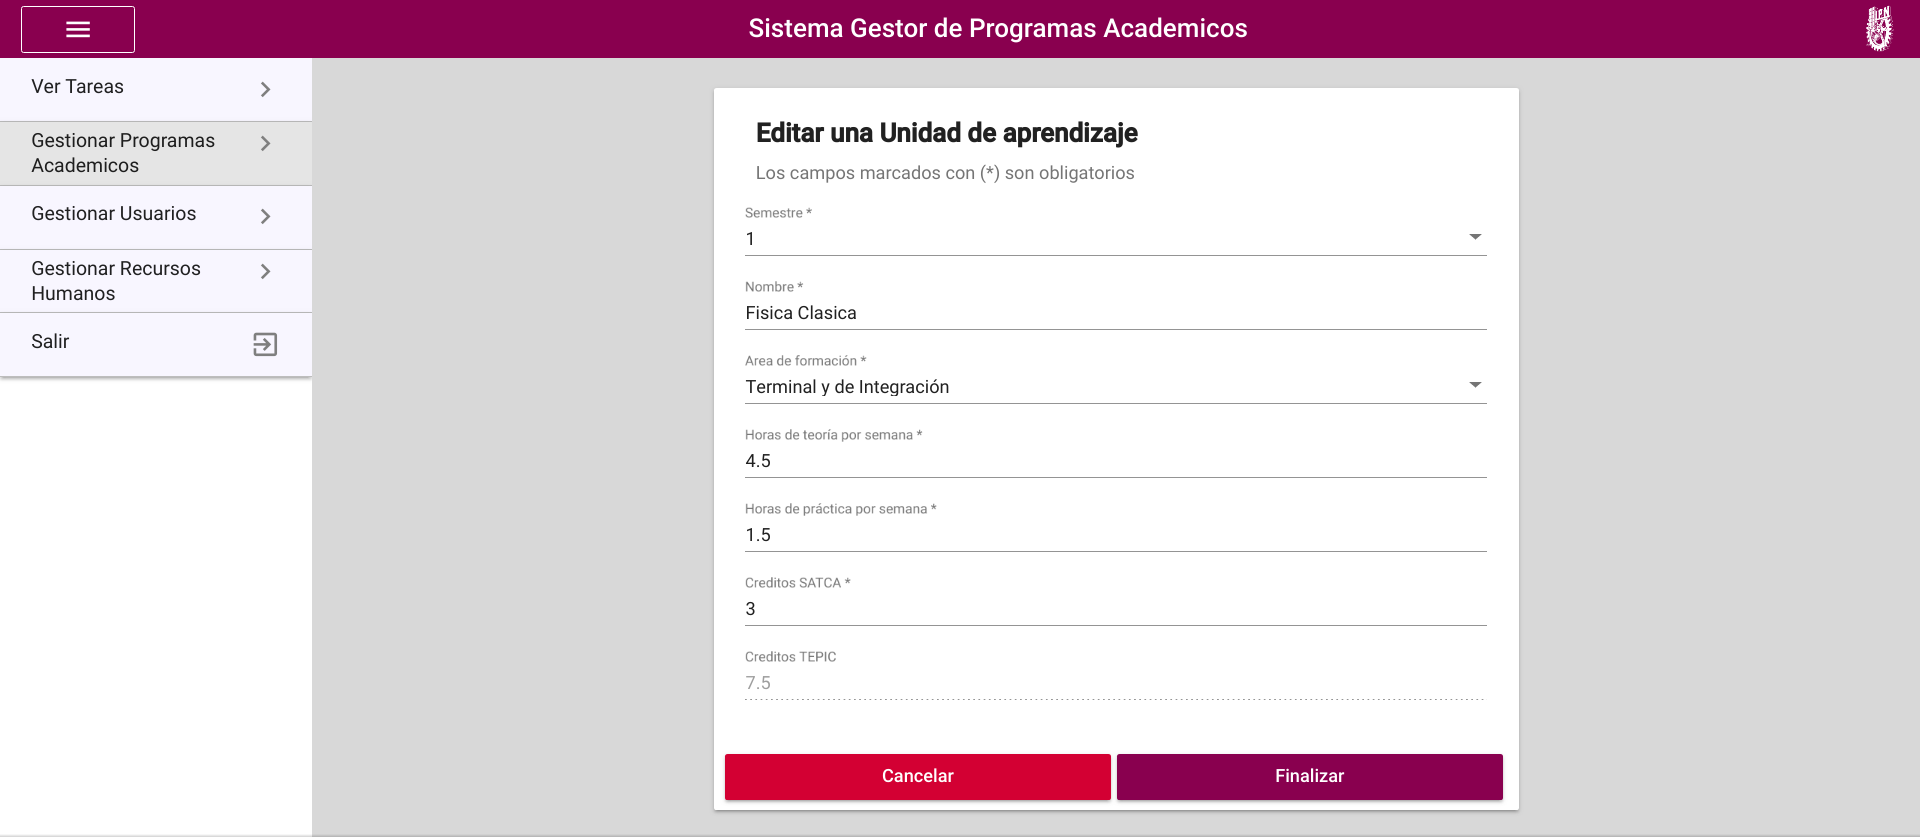
\includegraphics[width=0.7\linewidth]{images/GUA/editarUA}}
    \caption{Pantalla Editar Unidad de Aprendizaje}
    \label{editarUA}
\end{figure}
En la cual se cargarán los datos de la Unidad de Aprendizaje que el usuario haya seleccionado en la pantalla \hyperlink{consultarUA}{\textit{Consultar Planes de Estudios}}  y puede editar los campos que deseé.\\
Cuando modifique un dato y el nuevo valor no cumpla con el formato establecido para ese campo se muestra el siguiente mensaje:\\
\begin{figure}[H]
    \centering
    \hypertarget{invalidoE}{
\includegraphics[width=0.7\linewidth]{images/GUA/invalido}}
    \caption{Campo inválido: aparece cuando el formato o el tipo de dato es incorrecto}
    \label{invalidoE}
\end{figure}
Si un campo  obligatorio, es decir marcado con (*), es dejado en blanco, el sistema le muestra el siguiente mensaje:\\
\begin{figure}[H]
    \centering
    \hypertarget{requeridoE}{
\includegraphics[width=0.7\linewidth]{images/GUA/requerido}}
    \caption{Campo requerido: aparece cuando un campo obligatorio se dejo vacío}
    \label{requeridoE}
\end{figure}
Cuando haya terminado de realizar las modificaciones pertinentes presiona el botón \IUbutton{Finalizar} en la parte inferior de la pantalla para guardar lo cambios realizados.\\
\begin{figure}[H]
    \centering
    \hypertarget{finalizarBtnE}{
\includegraphics[width=0.7\linewidth]{images/GUA/finalizarBtn}}
    \caption{Botones para finalizar las operaciones de Edición}
    \label{finalizarBtnE}
\end{figure}
Si la operación pudo concluir sin errores se despliega el siguiente mensaje:\\
\begin{figure}[H]
    \centering
    \hypertarget{modificacion}{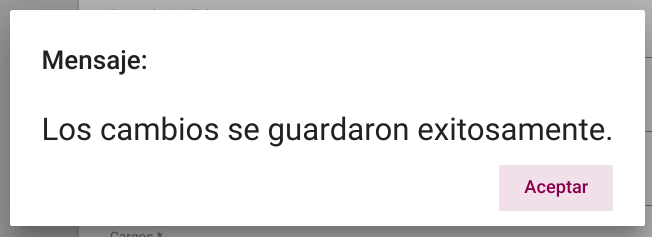
\includegraphics[width=0.7\linewidth]{images/GUA/modificacion}}
    \caption{Modificación exitosa: notifica del exito de la operación}
    \label{modificacion}
\end{figure}
En el caso de que ocurra un error aparecerá este otro:\\
\begin{figure}[H]
    \centering
    \hypertarget{errorE}{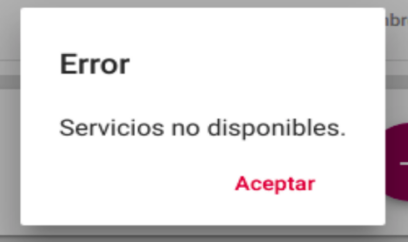
\includegraphics[width=0.7\linewidth]{images/GUA/error}}
    \caption{Error: Servicios no disponibles, aparece cuando ocurre un error en la conexión}
    \label{errorE}
\end{figure}
Si decide cancelar la operación y presiona el botón \IUbutton{Cancelar} aparece el siguiente mensaje para pedir su confirmación:\\
\begin{figure}[H]
    \centering
    \hypertarget{cancelarE}{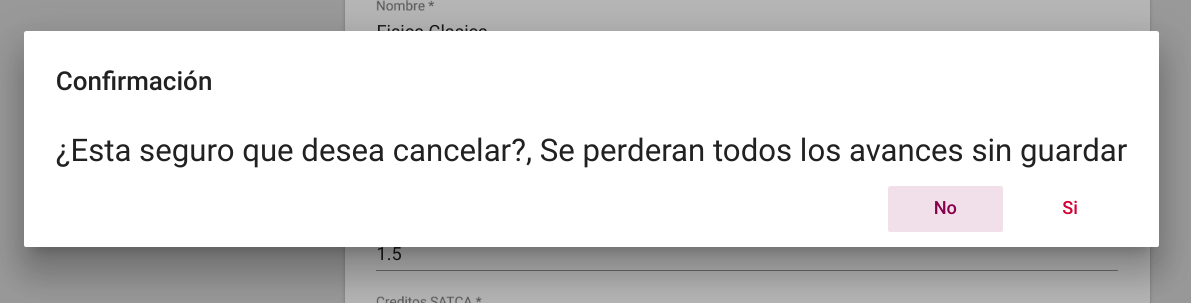
\includegraphics[width=0.7\linewidth]{images/GUA/cancelar}}
    \caption{Cancelación: permite finalizar la operacion sin guardar}
    \label{cancelarE}
\end{figure}
\newpage
\subsection{Eliminar Unidades de Aprendizaje}
Cuando el usuario presiona el botón \IUbutton{X}, el recuadro rojo, en la pantalla \hyperlink{consultarUA}{\textit{Consultar Planes de Estudios}} se muestra el siguiente mensaje solicitando confirmación:\\
\begin{figure}[H]
    \centering
    \hypertarget{EliminarUA}{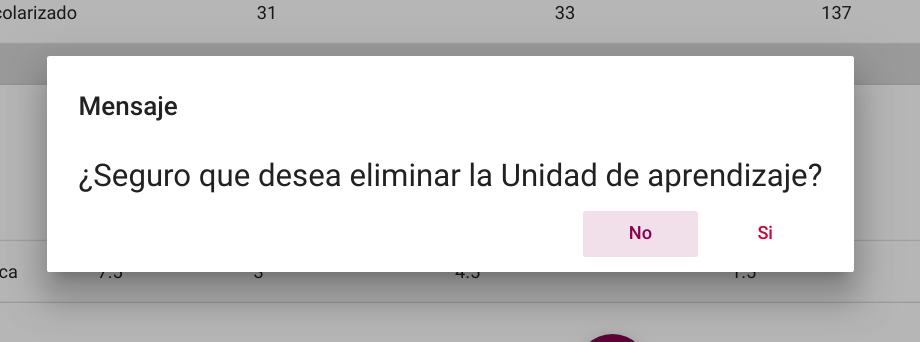
\includegraphics[width=0.7\linewidth]{images/GUA/EliminarUA}}
    \caption{Eliminar Unidad de Aprendizaje: solicita confirmación para eliminar permanentemente una Unidad de Aprendizaje}
    \label{EliminarUA}
\end{figure}
\newpage
\subsection{Consultar Programas de Estudios}
Cuando el usuario presiona el botón \IUbutton{ojo}, el recuadro purpura, en la pantalla \hyperlink{consultarUA}{\textit{Consultar Planes de Estudios}} se abre otra pestaña donde se muestra el pdf del Programa de Estudios de esa Unidad de Aprendizaje:\\
\begin{figure}[H]
    \centering
    \hypertarget{programaUA}{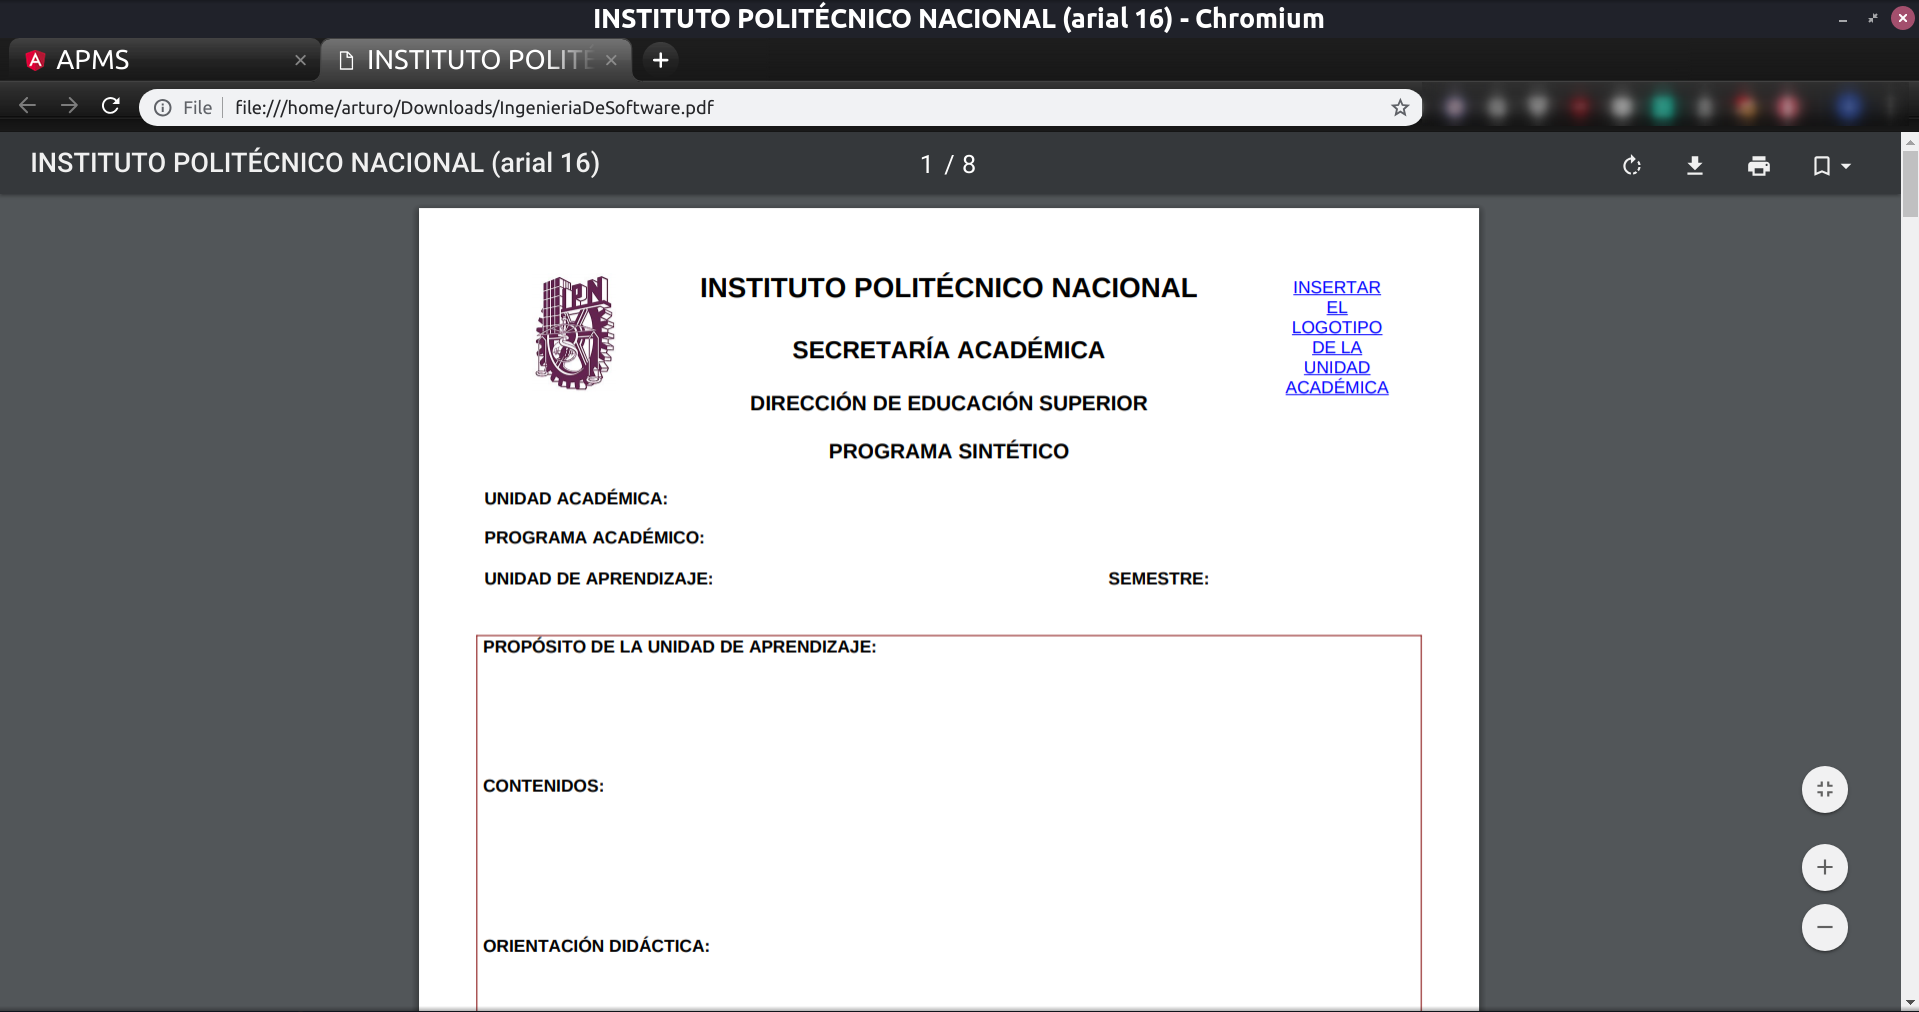
\includegraphics[width=0.7\linewidth]{images/GUA/programaUA}}
    \caption{Programa de Estudios: ejemplo de un Programa de Estudios}
    \label{programaUA}
\end{figure}